\documentclass[10pt,a4paper,onecolumn,openany]{book}
\usepackage[left=1.5cm,top=1.25cm,right=1.5cm,bottom=1.25cm]{geometry} 
\usepackage[utf8]{inputenc}
\usepackage[spanish]{babel}
%\usepackage{garamondx}
\usepackage{amsmath}
\usepackage{amsfonts}
\usepackage{amssymb}
\usepackage{makeidx}
\usepackage{graphicx}
\graphicspath{ {//home/alejandrocebrian/Escritorio/Recopilatorio} }
\usepackage{lmodern}
\usepackage{fourier}
\usepackage{soul} % para tachar palabras
\usepackage{multirow} 
\usepackage{subfigure}
\usepackage[hidelinks]{hyperref}	% Genera hipertextos dentro del pdf
\usepackage{stackrel}   % Permite escribir sobre los símbolos
\usepackage{floatrow}	% Permite poner a un lado los pies de imagen
\usepackage{csvsimple}
\usepackage{parskip}    % Permite modificar la distancia vertical.
\usepackage{indentfirst}% Permite modificar la indentación.
\setlength{\parindent}{15pt}
\setlength{\parskip}{0.5mm}
%\renewcommand{\baselinestretch}{0.5}
\usepackage{blindtext}
%\usepackage{natbib}
%\bibliographystyle{agsm}
\usepackage[table, dvipsnames]{xcolor}
\definecolor{hiperlightgray}{gray}{0.85}
\usepackage{listings}
\lstset{
	backgroundcolor=\color{hiperlightgray},   % Indica el color de fondo; necesita que se añada \usepackage{color} o \usepackage{xcolor}
	basicstyle=\scriptsize,
	language=bash,
	showstringspaces=false,
	formfeed=newpage,
	tabsize=4,
	commentstyle=\itshape,
	morekeywords={models, lambda, forms}}
\lstset{
	literate=
	{á}{{\'a}}1 {é}{{\'e}}1 {í}{{\'i}}1 {ó}{{\'o}}1 {ú}{{\'u}}1
	{Á}{{\'A}}1 {É}{{\'E}}1 {Í}{{\'I}}1 {Ó}{{\'O}}1 {Ú}{{\'U}}1
	{à}{{\`a}}1 {è}{{\`e}}1 {ì}{{\`i}}1 {ò}{{\`o}}1 {ù}{{\`u}}1
	{À}{{\`A}}1 {È}{{\'E}}1 {Ì}{{\`I}}1 {Ò}{{\`O}}1 {Ù}{{\`U}}1
	{ä}{{\"a}}1 {ë}{{\"e}}1 {ï}{{\"i}}1 {ö}{{\"o}}1 {ü}{{\"u}}1
	{Ä}{{\"A}}1 {Ë}{{\"E}}1 {Ï}{{\"I}}1 {Ö}{{\"O}}1 {Ü}{{\"U}}1
	{â}{{\^a}}1 {ê}{{\^e}}1 {î}{{\^i}}1 {ô}{{\^o}}1 {û}{{\^u}}1
	{Â}{{\^A}}1 {Ê}{{\^E}}1 {Î}{{\^I}}1 {Ô}{{\^O}}1 {Û}{{\^U}}1
	{œ}{{\oe}}1 {Œ}{{\OE}}1 {æ}{{\ae}}1 {Æ}{{\AE}}1 {ß}{{\ss}}1
	{ű}{{\H{u}}}1 {Ű}{{\H{U}}}1 {ő}{{\H{o}}}1 {Ő}{{\H{O}}}1
	{ç}{{\c c}}1 {Ç}{{\c C}}1 {ø}{{\o}}1 {å}{{\r a}}1 {Å}{{\r A}}1
	{€}{{\EUR}}1 {£}{{\pounds}}1 {ñ}{{\~n}}1 {¡}{{!`}}1 {¿}{{?`}}1}
\setlength{\parindent}{15pt}
\setlength{\parskip}{0.5mm}
%\renewcommand{\baselinestretch}{0.5}
\usepackage{multicol} 
\usepackage{enumitem} 
\usepackage[ruled,vlined]{algorithm2e}
\usepackage{float}
\usepackage{afterpage}
\usepackage{transparent}
\usepackage{eso-pic} % imagen de fondo
\newcommand\BackgroundPic{%
	\put(0,0){%
		\parbox[b][\paperheight]{\paperwidth}{%
			\vfill
			\centering
			{\transparent{0.3} 
\includegraphics[width=\paperwidth,height=\paperheight,%
				keepaspectratio]{Escudo.png}}%
			\vfill}}}
\usepackage{tabulary}
\usepackage[small]{caption} 
\author{Alejandro Cebrian del Valle}
\title{Biología: Curso general}
%\date{\vspace{-5ex}}
\begin{document}
\begin{titlepage}
	\AddToShipoutPicture*{\BackgroundPic}
	\centering
	\vspace*{\fill}
	\vspace*{0.5cm}
	\large Biblioteca personal de Educación \\
	\LARGE \textbf{Biología: elementos fundamentales\\}
	\vspace*{2cm}
	\large  Alejandro Cebrian y del Valle \\
	\vspace*{2cm}
	\today
	\vspace*{\fill}
\end{titlepage}
\afterpage{\null\newpage}
\newpage
\tableofcontents
\part{Introducción a la biología y ciencias afines}
\part{Bioquímica}
\part{Botánica y Fisiología vegetal}
\part{Fisiología}
\part{Genética}
\part{Microbiología}
\chapter{Ultraestructura interna}
\section{Citoplasma}
El citoplasma está compuesto en un 70\% por agua, dónde se encuentran en solución coloidal una gran cantidad de macromoléculas u otras biomoléculas o bioelementos, con una presión oncótica u osmótica de 2 atmósferas. En el citoplasma, además, se encuentran presentes las enzimas bacterianas necesarias para su metabolismo y chaperonas (proteínas que ayudan a una proteína a alcanzar su plegamiento correcto). Así mismo se hallan proteínas con una función estructural, que dan forma a la célula, asimilándose al citoesqueleto de eucariotas. Algunas proteínas son:
\begin{itemize}[itemsep=0pt,parsep=0pt,topsep=0pt,partopsep=0pt]
	\item \textbf{FtsZ} (similar a la tubulina): tienen función en la división celular. Se encuentra en numerosas especies de Bacteria y Archaea.
	\item \textbf{MreB} (similar a la actina): dan la forma a la célula. Se encuentran en muchos géneros de bacilos.
	\item \textbf{Crescentina}: (similar a filamentos internos) dan forma a la célula. Se encuentra en especies como el \textit{Caulobacter crecentus}.
\end{itemize}

En el citoplasma se encuentran, además, orgánulos y el nucleoide. El nucleoide es el área del citoplasma donde se coloca el material genético (normalmente, un cromosoma circular) y plásmidos. Estos últimos son cadenas de DNA no vitales, pero que confieren al individuo ventajas adaptativas como resistencia a antibióticos, a daños or metales pesados o la incorporación al metabolismo de otros compuestos, como el plásmido \textit{Tol} (tolueno) de \textit{Pseudomona}. El cromosoma se encuentra, como en eucariontes, superenrollado, pero en este proceso no participan histonas.

Los ribosomas son el único orgánulo celular compartido con los tres dominios celulares. Con la misma función en todos los individuos, el bacteriano es de 70S, con una subunidad menor de 30S (compuesto por 21 proteinas y RNAr de 16S) y una mayor de 50S (compuesto por 34 proteínas y dos RNAr, uno de 23S y otro de 5S).

Otro tipo de orgánulo bacteriano son las inclusiones. Las inclusiones son gránulos de material orgánico o inorgánico envuelto o no por una membrana no unitaria (formadas por proteínas, lipoproteínas o glicoproteínas). Se generan, normalmente, bajo condiciones determinadas de crecimiento. Pueden ser:
\begin{itemize}[itemsep=0pt,parsep=0pt,topsep=0pt,partopsep=0pt]
	\item \textbf{Orgánicas}: de polisacáridos, de poli-$\beta$-hidroxialcano o cianoficina
	\item \textbf{Inorgánicas}: polifosfato o de azufre elemental. 
\end{itemize}

Algunos otros orgánulos no rodeados por membrana son las vesículas de gas, clorosomas, carboxisomas o magnetosomas. Como única excepción a la no presencia de orgánulos rodeados por membrana unitaria son los tilacoides de las cianobacterias.
\subsection{Inclusiones orgánicas}
Pueden ser:
\begin{itemize}[itemsep=0pt,parsep=0pt,topsep=0pt,partopsep=0pt]
	\item \textbf{Polisacarídicas}: de glucógeno (ósido de reserva animal) o de almidón (ósido de reserva vegetal). Ambos polímeros de glucosasirven como reservorio de carbono. Se comienzan a sintetizar cuando en el medio hay falta de nitrógeno. Cuando se restituye este elemento, se forman las proteínas con el carbono almacenado.
	\item De \textbf{poli-$\beta$-hidroxialcanoatos} (PHA): se encuentran entre ellos:
	\begin{itemize}[itemsep=0pt,parsep=0pt,topsep=0pt,partopsep=0pt]
		\item \textbf{Poli-$\beta$-hidroxibutirato} (PHB) polímero de ácido 3-hidroxibutírico unidos por enlace éster. Sirve como reservorio de carbono antes de la esporulación en \textit{Pseudomona} y \textit{Bacillus}.
		\item \textbf{Otros}, con función de bioplásticos (en el organismo vivo se utilizan como reserva de carbono), son copolímeros de poli-$\beta$-hidroxibutírico y poli-$\beta$-hidroxivalérico.
	\end{itemize}
	\item \textbf{Cianoficina}: presente únicamente en cianobacterias, como la Anaystis nidulans, son polímeros de aspartato con ramificaciones de arginina, unidos por enlaces peptídicos. Estas inclusiones, cuya generación se produce ante la falta en el medio de algún nutriente, se utilizan como reserva de carbono y nitrógeno.
\end{itemize}
\subsection{Inclusiones inorgánicas}
De las más conocidas son:
\begin{itemize}[itemsep=0pt,parsep=0pt,topsep=0pt,partopsep=0pt]
	\item \textbf{Inclusiones de polifosfato}: se dan en los géneros Lactobacillus y Spirilum. Se conocen también como gránulos de volutina o metacromáticos. Sirven de reserva de fosfato, produciéndose ante la falta de azufre.
	\item \textbf{Inclusiones de azufre}: observables en las bacterias verdes y en las quimiolitotrofas. En ambos casos, son acumulaciones temporales de azufre elemental que se da por un proceso lento de oxidación a sulfato ($SO_4^{2-}$). Se usa, en el caso de bacterias verdes, para obtener poder reductor, y en el caso de quimiolitotrofos, para obtener poder reductor y energía.
\end{itemize}
\subsection{Vacuolas de gas}
Estos orgánulos no presentan límite de membrana unitaria. Se hallan presentes en algunas procariotas, sobre todo acuáticas, siendo su función la de permitir al organismo moverse en la vertical hacia hábitats más propicios (más luz, nutrientes,$\dots$). Son agregados de un gran número de estructuras pequeñas huecas cilíndricas o fusiformes. Las cianobacterias con vesículas de gaspresentan una membrana especial, permeable a los gases, pero no al agua. De esta forma, al reducir su contenido en gas, desciende en profundidad; y al aumentar la cantidad de gas, ascienden.
\part{Parasitología}
\chapter{Introducción}
La parasitología es una rama de la Biología que estudia el parasitismo, realción ecológica entre dos seres de distinta especia (relación esterotípica o anisoespecífica) denominados hospedador, que proporciona un medio; y se relaciona con un parásito, ecuariota que desarrolla una dependencia metabólica con respecto al hospedador, mediante respuesta inmune. Entre hospedador y parásito se da una relación semántica y coevolutiva, por medio de adpatación. La relación de parasitismo puede prosperar o fracasar según el medio externo.

La parasitología sanitaria consiste en el estudio de los parasitismos que afectan al ser humano y que pueden tener repercusiones tanto para la salud individual que las padece como las poblaciones que les afecta. Mediante el estudio tanto de la morfología y biología de los parásitos como de las enferemedades que originan (patología y sintomatología) fijando las bases para su control.
\section{Definiciones}
\paragraph{Parásito}\footnote{\textit{al lado de la comida}}: a nivel biológico, animal que vive a expensas de otro. Forman en torno a dos tercios de la fauna del planeta. Comienzan a surgir a partir de organismos de vida libre, siendo los primeros los \textit{Unos} (tenias) en el Paleozoico, se expanden en número en el Cretácico y era Terciaria, dandose fenómenos de adaptaciones a tiempo real (amebas anfizoicas). De origen polifilético y evolutivo y temporal distintos, se clasifican:
\begin{itemize}[itemsep=0pt,parsep=0pt,topsep=0pt,partopsep=0pt]
	\item Según su habitat ojetivo:
	\begin{itemize}[itemsep=0pt,parsep=0pt,topsep=0pt,partopsep=0pt]
		\item \textbf{Fitoparásitos}: o plagas, son parásitos de plantas.
		\item\textbf{Zooparasitos}: parásitos de animales. Se subdividen:
		\begin{itemize}[itemsep=0pt,parsep=0pt,topsep=0pt,partopsep=0pt]
			\item \textbf{Ectoparásitos}: se localizan en el exterior. Pueden ser Hematófagos o no hematófagos.
			\item\textbf{Endoparásitos}: habitan en el interior del hospedador. Son:
			\begin{itemize}[itemsep=0pt,parsep=0pt,topsep=0pt,partopsep=0pt]
				\item Intestinales
				\item Subcutáneos
				\item Cavitarios (en el interior de órganso).
				\item Endocelulares
				\item Cenozoicos (en el interior del núcleo celular).
				\item Erraticos (Se mueven por el hospedador. Se pueden diferenciar de localización errática en tanto que alude a parásitos que no están en su hábitat habitual).
			\end{itemize}
		\end{itemize}
	\end{itemize}
	\item Según su tiempo de contacto:
	\begin{itemize}[itemsep=0pt,parsep=0pt,topsep=0pt,partopsep=0pt]
		\item \textbf{Permanente}: (piojos,$\dots$) lleva a cabo todo su ciclo biológico en un mismo hospedador: viviendo, creciendo y reproduciéndose en él.
		\item\textbf{Temporal}: (pulgas, etc.) el parásito vive en el ambiente del hospedado, próximo a él, pero sólo accede a este cuando precisa de cierta necesidad.
		\item\textbf{Estacional}: (mosquitos, $\dots$) sólo está presente en ciertas épocas del año.
		\item\textbf{Facultativos}: (\textit{Lucilia} spp, etc) el parásito puede vivier de forma libre o en forma parasitaria en alguno de los momentos de su vida.
	\end{itemize}
	\item Según los hospedadores intermedios en su ciclo vital:
	\begin{itemize}[itemsep=0pt,parsep=0pt,topsep=0pt,partopsep=0pt]
		\item \textbf{Monoxenos}: sólo presenta un hospedador.
		\item\textbf{Heteroxenos}: presenta varios hospedadores intermedios.
		\item\textbf{Poliheteroxenos}: presenta múchos hospedadores intermedios.
	\end{itemize}
	\item Según su especificidad:
	\begin{itemize}[itemsep=0pt,parsep=0pt,topsep=0pt,partopsep=0pt]
		\item \textbf{Estenoxeno}: (piojos, $\dots$) requieren unas condiciones muy concretas que provoca que se desarrollen sólo en una o muy pocas especies.
		\item\textbf{Eurixeno}: (\textit{Toxoplasma gondii}, etc.) tiene requerimientos poco específicos, por lo que puede desarrollarse en varias especies.
	\end{itemize}
\end{itemize}
\paragraph{Hospedador}: animal que proporciona un ambiente al parásito. Se clasifican:
	\begin{itemize}[itemsep=0pt,parsep=0pt,topsep=0pt,partopsep=0pt]
		\item \textbf{Definitivo}: hospedador en el que el parásito está en forma adulta y es capaz de reproducirse sexualmente.
		\item\textbf{Intermedio}: hospedador en el que el parásito está en forma larvaria y es capaz de reproducirse asexualmente.
		\item\textbf{Paraténica}: hospedador no necesario en el que el parásito permanece en un determinado estado y en el que no se reproduce, alargando su ciclo vital.
		\item\textbf{Reservorio}: hospedador vertebrado no humano que actúa como hospedador definitivo y supone una provisión de parásitos en la naturaleza (\textit{Leishmania} spp y el perro).
		\item\textbf{Vector}: hospedador invertebrado que actúa como hospedador intermedio\footnote{Se daría reproducción asexual} y como medio de transporte del parásito\footnote{Excepto \textit{Plasmodium} y el mosquito \textit{Anopheles}, ya que existe reproducción sexual en él} (\textit{Plasmodium} y la mosca tse-tse).
		\begin{itemize}[itemsep=0pt,parsep=0pt,topsep=0pt,partopsep=0pt]
			\item \textbf{Transmisor mecánico} o \textbf{portador}: hospedador donde no se da ningún tipo de reproducción, sólo dándose un movimiento entre dos puntos. Se usa con ectoparásitos.
		\end{itemize}
	\end{itemize}
\paragraph{Ciclo biológico}: conjunto de sucesos por los que pasa un parásito desde una fase determinada hasta que vuelve a esa fase. Existen distintos tipos:
\begin{itemize}[itemsep=0pt,parsep=0pt,topsep=0pt,partopsep=0pt]
	\item \textbf{Directo}: no existen hospedadores intermedios. Pueden ser:
	\begin{itemize}[itemsep=0pt,parsep=0pt,topsep=0pt,partopsep=0pt]
		\item \textbf{Saprozoico}: se transmite por agua o suelo, vehiculizado por estos.
		\item\textbf{No saprozoico}: se transmite de un hospedador a otro.
	\end{itemize}
	\item\textbf{Indirecto}: existen uno o varios hospedadores intermedios.
	\item\textbf{Facultativos}: Puede tener o no hospedadores intermedios.
	\item\textbf{Autoheteroxenos}: en el mismo hospedador se desarrolla todo el ciclo vital del parásito. (\textit{Trichinella} spp).
\end{itemize}
\paragraph{Ciclo epidemiológico}: referido a un hospedador, conjunto de sucesos por los que pasa un parásito al salir de un hospedador hasta que vuelve al mismo.
\paragraph{Agente etiológico o causal}: parásito, en cualquiera de sus formas, pudiendo darse que el mismo agente etiológico (parásito) esté en uno u otro estado dependiendo del hospedador. Se pueden llevar dos tipos de diagnósticos:
\begin{itemize}[itemsep=0pt,parsep=0pt,topsep=0pt,partopsep=0pt]
	\item \textbf{Directo}: búsqueda del parásito en el hospedador en cualquiera de las formas del ciclo vital de este.
	\item\textbf{Indirecto}: búsqueda de anticuerpos ante el parásito y de otros marcadores de respuesta inmune (más limitado por inespecificidad y poca antigenicidad).
\end{itemize}
\paragraph{Fuente de infección}: medio que lleva al parásito hasta el siguiente hospedador.
\paragraph{Vía de infección}: canal por el que llega el parásito al hospedador:
\begin{itemize}[itemsep=0pt,parsep=0pt,topsep=0pt,partopsep=0pt]
	\item Oral.
	\item Parenteral (a través de la piel y hacia la sangre).
	\item Congénita o placentaria.
	\item Venérea.
	\item Galactógena.
\end{itemize}
\section{Epidemiología}
\subsection{Introducción y definiciones}
\paragraph{Epidemiología}: ciencia que estudia el conjunto de conocimientos relativos a las enfermedades de las poblaciones humanas o comunidades más que la individuales. Estudia el conjunto de factores que determinan frecuencia y distribución de las enfermedades.
\paragraph{Prevalencia}: proporción de individuos que albergan el parásito (enfermos nuevos y antiguos) en una población determinada. Se expresa en porcentaje:
\begin{center}
	\begin{math}
		\mbox{Prevalencia} = \dfrac{\mbox{Nº parasitados}}{\mbox{Población total}} \cdot 100
	\end{math}
\end{center}
\paragraph{Incidencia}: casos nuevos de parasitosis en una población y periodo temporal. Se expresa como casos por 100 000 habitantes y año.

La prevalencia depende de la incidencia y duración de las parasitosis en tanto que alta incidencia y/o una enfermedad crónica aumnetan la prevalencia, mientras que parasitosis poco incidentes y/o de corta duración (rápida curación o alta mortalidad), la hacen descender.

\paragraph{Endemia/enzootia}: enfermedad constante en cieratas épocas y regiones por influencia de una causa local (gran número de hospedadores, etc.)
\paragraph{Hiperendemia/hiperenzootia}: endemia de alta prevalencia, originada por descontrol de una endemia.
\paragraph{Epidemia/Epizootia}: infección accidental transitoria que afecta al mismo tiempo y en la misma región a un gran número de individuos.
\paragraph{Pandemia}: epidemia que afecta a gran número de regiones.
\subsection{Factores determinantes}
Entre los factores que pueden determinar la distribuciónd e la enfermedad, se pueden agrupar en ambientales y derivados de la actividad humana.
\begin{itemize}[itemsep=0pt,parsep=0pt,topsep=0pt,partopsep=0pt]
	\item \textbf{Ambientales}:
	\begin{itemize}[itemsep=0pt,parsep=0pt,topsep=0pt,partopsep=0pt]
		\item \textbf{Bióticos}: se relacionan con la vegetación, que sirve de refugio a formas de vida libre o determina la presencia o no de ciertos hospedadores; y faunta, comunidades que viven juntos de especies distintas que se infectan a la vez y presencia de vectores en el ecosistema.
		\item\textbf{Abióticos}: del biotopo. Son:
		\begin{itemize}[itemsep=0pt,parsep=0pt,topsep=0pt,partopsep=0pt]
			\item \textbf{Climáticos}: como temperatura (altas temperaturas favorecen los ciclos de vida libre y los ciclos de transmisión por los artrópodos), viento (algunos vectores son incapaces de vivir en zonas con altos flujos de aire) o humedad (la alta humedad favorece los ciclos de vida libre al evitar la desecación y favorecer una gran vegetación que dé refugio y zonas sombrias que eviten la deshidratación del parásito).
			\item\textbf{Edáficas}: condicionan, la aridez o compactación del suelo, la supervivencia de ciclos de vida libre.
			\item\textbf{Hídricos}: el pH, turbidez, cantidad de oxígeno disuelto y materia orgánica, así como régimen de turbulencias, condicionan la vida de ciclos de vida libre y la posibilidad de infectar a un hospedador.
		\end{itemize}
	\end{itemize}
	\item\textbf{Antropogénicos}:
	\begin{itemize}[itemsep=0pt,parsep=0pt,topsep=0pt,partopsep=0pt]
		\item \textbf{Dependientes del nivel de desarrollo}: uso de suelos, disponibilidad de alimentos y agua potable, condiciones de vivienda, sanidad, escolaridad, etc.
		\item\textbf{Dependientes de la actividad humana}: construcción de grandes infraestructuras, colonización de áreas poco pobladas y deforestación, existencia de programas sanitarios, proximidad de animales (zoonosis), incremento del comercio y viajes, cambios demográficos (mayor población urbana que conlleva hacinamiento y escasez de servicios).
		\item\textbf{Existencia de conflictos armados}: dado que determina cambios ambientales y el desplazamiento forzoso de gran número de personas (hacinamiento, falta de servicios y salubridad).
	\end{itemize}
\end{itemize}

Todos estos factores determinan la distribución mayoritaria de las parasitosis en regiones tropicales: las condiciones de subdesarrollo determinan el desarrollo de parásitos que lastran el desarrollo económico.
\section{Respuesta inmune}
La respuesta inmune frente a los parásitos es muy compleja y rara vez suele ser tan sólida como la que se desarrolla frente a bacterias y virus\footnote{Excepto las leishmaniosis cutáneas que curan de forma espontánea y confieren inmunidad.}. Se puede llegar a cierta inmunidad ante gran cantidad de exposiciones, por ejemplo, los infectados por determinadas cepas son resistentes a cepas homólogas pero no a heterólogas.

Así mismo, en ciertas ocaciones, la respuesta inmune no sólo resulta inútil frente al parásito, sino que también es lesiva para el hospedador (inmunopatología), pudiendose dar fenómenos de alergias e hipersensibilidad (helmintos), destrucción de células sanas (hemolisis por antígenos adsorbidos de \textit{Plasmodium}), o formación de granulomas y fibrosis en órganos (\textit{Schistosoma}). Además, el propio parásito se ha dotado de estrategias para evitar o evadir la respuesta inmune.
\subsection{Mecanismos de evasión}
La respuesta inmunitaria se lleva a cabo mediante dos mecanismos:
\begin{itemize}[itemsep=0pt,parsep=0pt,topsep=0pt,partopsep=0pt]
	\item \textbf{Inmunidad natural innata}: es inespecífica (se desencadenan las mismas reacciones frente a distintos patógenos) y se produce en el momento de la entrada del parásito. Consiste en fagocitosis y reacciones inflamatorias de carácter humoral.
	\item\textbf{Respuesta adaptativa}: es de tipo específico (a distintos patógenos, distintos procesos), ligadas a ciertas células (linfocitos y células presentadoras de antígenos, leucocitos y anticuerpos), pudiendo ser de carácter celular, dependiendo de linfocitos T, o humoral, de linfocitos B. Actúan tiempo después de la entrada del parásito, se incrementan y persisten actuando por procesos complejos y únicamente frente a especias que indujeron su activación.
\end{itemize}

Dada la diferencia a nivel estructural, bioquímico, patogénico y de ciclo biológico, no se puede formar una respuesta inmune única. Aun así, según la localización del parásito, se pueden distinguir:
\begin{itemize}[itemsep=0pt,parsep=0pt,topsep=0pt,partopsep=0pt]
	\item Parásitos que viven en el entorno intracelular, generan una respuesta fundamentalmente celular (protozoos).
	\item Parásitos que viven en el medios extracelular y en sangre, inducen respuestas humorales.
\end{itemize}

Los mecanismos de evasión de la respuesta inmune más frecuentes son:
\begin{itemize}[itemsep=0pt,parsep=0pt,topsep=0pt,partopsep=0pt]
	\item \textbf{Evasión del reconocimiento}: el parásito modifica de forma frecuente sus antígenos de superficie, volviendo ineficaces a los anticuerpos formados frente al parásito (tripanosomas africanos).
	\item\textbf{Enmascaramiento antigénico}: para evitar la dispersión del parásito por el organismo, esta los tapiza formando una membrana que impide el contacto con células inmunes y por ello, la respuesta inmune (quistes hidatídicos).
	\item\textbf{Encapsulamiento}: el parásito penetra en una célula, a la que modifica (formación de más retículo endoplásmico, creación de una cubierta,$\dots$) haciendola más fibrosa, como un quiste, y transformandola en una <<célula nodriza>> que protege al parásito (\textit{Trichinella}).
	\item\textbf{Modificación de la expresión antigénica}: según el estado de desarrollo, la fase del parásito en cada momento, tendrá distintos marcadores celulares (\textit{Plasmodium} varía sus antígenos en el momento de entrada al hepatocito, donde se reproduce asexualemnte, a su salida de éste y en el momento de entrada al eritrocito).
	\item\textbf{Adaptación a vivir en <<paraísos parasitarios>>}: el parásito vive en una región del organismo donde no llega la respuesta inmune (\textit{Toxoplasma gondii} y su colonización del Sistema Nervioso Central (SNC)).
	\item\textbf{Adaptación a vivir en células inmunes}: el parásito segrega enzimas que permiten vivir y multiplicarse en vacuolas líticas leucocitarias (\textit{Leishmania}).
	\item\textbf{Cubiertas}: posesión de un glicocálix o tegumento graso que protege frente a mecanismos citotóxicos de macrófagos y neutrófilos (helmintos).
\end{itemize}
\subsection{Inmunodiagnóstico}
Las características exigibles a cualquier prueba diagnóstica son:
\begin{itemize}[itemsep=0pt,parsep=0pt,topsep=0pt,partopsep=0pt]
	\item \textbf{Sensibilidad}: capacidad de detección de casos positivos ante cantidades mínimas de marcador.
	\item\textbf{Especificidad}: capacidad de detección de casos negativos, eliminando reacciones cruzadas.
	\item\textbf{Reproducibilidad}: capacidad de que tantas veces se repita el experimento, el resultado no varie.
	\item Facilidad de realización, rapidez y bajo coste.
\end{itemize}
A estas características se le ha de añadir la definición de un título límite del marcador que indique la presencia de parasitosis.

El diagnóstico inmunológico es un tipo de diagnóstico indirecto que complementa al directo o morfológico, pero no lo sustituye. De gran utilidad cuando el parásito no es fácilmente localizable o no hay formas de eliminación. Existen varios tipos:
\begin{itemize}[itemsep=0pt,parsep=0pt,topsep=0pt,partopsep=0pt]
	\item Detección de antígenos específicos.
	\item Detección de antígenos solubles.
	\item Detección de inmunocomplejos circulantes.
	\item Exploración de inmunidad mediada por células (citoquinas, interleuquinas, interferones, linfoblastos, $\dots$)
\end{itemize}
Las técnicas más usadas son:
\begin{itemize}[itemsep=0pt,parsep=0pt,topsep=0pt,partopsep=0pt]
	\item \textbf{Reacciones de precipitación}: inmunoelectroforesis, inmunodifusióon radial (Mancini), doble difusión, contrainmunoelectroforesis, etc.
	\item\textbf{Reacciones de aglutinación}: aglutinación directa, hemoaglutinación, aglutinación con látex, Pentonita.
	\item\textbf{Marcadores}: inmunofluorescencia, enzimoimnunoanálisis (ELISA y variantes), radioinmunoanálisis.
\end{itemize}
\section{La enfermedad parasitaria}
En el caso del parasitismo, de la interacción hospedador-parásito, pueden darse 4 supuestos:
% Please add the following required packages to your document preamble:
% \usepackage{multirow}
\begin{table}[H]
	\begin{tabular}{cccc}
		&  & \multicolumn{2}{c}{Hospedador} \\
		&  & \multicolumn{1}{c|}{Vive} & Muere \\ \cline{3-4} 
		\multirow{2}{*}{Parásito} & \multicolumn{1}{c|}{Vive} & \multicolumn{1}{c|}{\begin{tabular}[c]{@{}c@{}}Parasitismo próspero: parásito vive y\\ hospedador lo tolera\end{tabular}} & \begin{tabular}[c]{@{}c@{}}Parásito se establece pero \\ mata al hospedador\end{tabular} \\ \cline{2-4} 
		& \multicolumn{1}{c|}{Muere} & \multicolumn{1}{c|}{\begin{tabular}[c]{@{}c@{}}Parásito se establece y\\ el hospedador lo mata\end{tabular}} & Parásito no se establece
	\end{tabular}
	\caption{Cuadro de relaciones de parasitismo. \label{table:PARASIT:EnferParasRelac}}
\end{table}

En una relación de parasitismo se define:
\begin{itemize}[itemsep=0pt,parsep=0pt,topsep=0pt,partopsep=0pt]
	\item \textbf{Infección inaparente}: los parásitos viven en el hospedador sin causar daño aparente durante periodos largos o recidivas(en el caso de los helmintos, sólo se ven síntomas en caso de que gran número de ellos estén; o en el caso del paludismo, las recidivas cada 48 o 72 horas).
	\item\textbf{Portador sano}: estado del portador durante la infección inaparente, no manifestando signos ni síntomas, dado que el daño tisular se realiza a la misma velocidad de recuperación, con posibilidad de transmisión del parásito.
	\item\textbf{Parasitismo}: relación en equilibrio entre parásito y hospedador sano o portador.
	\item\textbf{Parasitosis}: enfermedad parasitaria provocada por la ruptura del equilibrio del parasitismo. Aun sin daños en el hospedador, el parásito es casi siempre un patógeno.
	\item\textbf{Patogenicidad}: capacidad de un parásito de producir daño a un hospedador, generando una enfermedad.
\end{itemize}

Los parásitos, como todo ser vivo de la escala zoológica, tiene un nombre genérico y otro específico que lo identifica, escribiendos siempre en cursiva o subrayado, el latín y con el género empezando en mayúscula. Las enfermedades producidas por los parásitos se nombran como el género del parásito que la produce acabado en <<-\textit{osis}>> (o -\textit{asis} o -\textit{iasis}). En cuanto a las parasitosis, se clasifican:
\begin{itemize}[itemsep=0pt,parsep=0pt,topsep=0pt,partopsep=0pt]
	\item \textbf{Antroponosis}: parasitósis exclusivas del ser humano.
	\item\textbf{Zoonosis}: parasitosis exclusivas de animales no humanos.
	\item\textbf{Antropozoonosis}: parasitosis que afectan por igual a todos los animales, incluidos humanos.
\end{itemize}
\subsection{Factores condicionantes de la patogenia}
Se pueden distinguir entre factores intrínsecos (del parásito) y extrínsecos (del hospedador):
\begin{itemize}[itemsep=0pt,parsep=0pt,topsep=0pt,partopsep=0pt]
	\item \textbf{Intrínsecos}:
	\begin{itemize}[itemsep=0pt,parsep=0pt,topsep=0pt,partopsep=0pt]
		\item \textbf{Grado de infección}: número de parásitos que se asientan en el hospedador. Cuanto mayor sea, más patógeno será el parásito.
		\item\textbf{Capacidad de multiplicación del parásito}.
		\item\textbf{Virulencia}: capacidad del parásito de producir daño.
		\item\textbf{Localización del parásito}: depende de la localización puntual del parásito en caso de migrar, dandose mayor estimulación antigénica en sangre y tejidos que en el intestino.
	\end{itemize}
	\item\textbf{Extrínsecos}:
	\begin{itemize}[itemsep=0pt,parsep=0pt,topsep=0pt,partopsep=0pt]
		\item \textbf{Edad}.
		\item\textbf{Estado funcional}: embarazo o lactancia exacerban los síntomas y daños.
		\item\textbf{Estado nutricional}.
		\item\textbf{Estado inmunitario}.
	\end{itemize}
\end{itemize}

Así, se definen los siguientes términos:
\begin{itemize}[itemsep=0pt,parsep=0pt,topsep=0pt,partopsep=0pt]
	\item \textbf{Periodo de incubación}: periodo de tiempo transcurrido entre el contagio y la aparición de síntomas y signos.
	\item\textbf{Periodo prepatente}: tiempo que transcurre desde el contagio hasta la eliminación de formas parasitarias de transmisión.
	\item\textbf{Periodo patente o de estado}: periodo de tiempo en elq ue la enfermedad es manifiesta y se eliminan formas de diseminación.
	\item\textbf{Periodo postpatente}: tiempo de ausencia de sintomatología y descenso de formas de eliminación.
	\item\textbf{Etiología}: causa de la enfermedad.
	\item\textbf{Patogénia}: dinámica de la enfermedad, estudio de la interacción parásito-hospedador.
	\item\textbf{Sintomatología}: conjunto de signos\footnote{manifestaciones cuantificables y objetivas.} y síntomas\footnote{manisfestaciones subjetivas.} de la enfermedad. En el caso de las parasitosis, la sintomatología, por ser vaga y fácilmente confundible, no es definitoria de enfermedad, necesitando confirmar diagnósticos mediante laboratorio.
\end{itemize}
\subsubsection{Acción patogénica del parásito}
Los parasitos pueden causar daño al hospedador mediante distintas acciones:
\begin{itemize}[itemsep=0pt,parsep=0pt,topsep=0pt,partopsep=0pt]
	\item \textbf{Mecánicas}: según el volumen, número y localización de los parásitos pueden ser:
	\begin{itemize}[itemsep=0pt,parsep=0pt,topsep=0pt,partopsep=0pt]
		\item\textbf{De presión}: quistes hidatídicos, cisticercosis cerebrales, etc.
		\item\textbf{De bloqueo}: filarias linfáticas, ascaris intestinales, $\dots$
	\end{itemize}
	\item\textbf{Traumática}: ruptura de tejidos por penetración, migración o asentamiento del parásito.
	\item\textbf{Expoliadora}: sustracción de nutrientes de tipo general o específico.
	\item\textbf{Toxicológica}: dada por sustancias producidas por el vector (hinchazón ante la picadura, etc.) o metabolitos del parásito (sarcocistina, un neurotóxico del parásito \textit{Sarcocystis}).
	\item\textbf{Vehiculadora}: transporte de gérmenes de un sitio a otro (infección secundaria), pudiendo ser desde el medio externo o interno.
	\item\textbf{Estimulación de reacciones hísticas}: inflamaciones, encapsulamiento fibrosos o eosinofilia (helmintos). Resultan en:
	\begin{itemize}[itemsep=0pt,parsep=0pt,topsep=0pt,partopsep=0pt]
		\item\textbf{Hipertrofia}: aumento del tamaño del órgano.
		\item\textbf{Hiperplasia}: aumento de la función del órgano.
		\item\textbf{Neoplasia}: aumento de la división celular en el órgano.
	\end{itemize}
\end{itemize}
\subsection{Importancia socioeconómica}
A pesar del gran porcentaje de población (33 \%) que sufre estas enfermedades, son enfermedades desatendidas.
\begin{multicols}{2}
	Las parasitosis tiene efecto a nivel económico en tanto pérdida de mano de obra (incapacidad o muerte), como aumento del gasto sanitario y pérdidas por absentismo laboral, así como de perdida de productividad en el caso de las zoonosis, por muerte del ganado y pérdida de fuerza de tiro. El aumento de las zoonosis también genera un aumento de las antropozoonosis, especialmente virulentas en ninños (con mayor contacto y menor desarrollo inmune), que lastra el aumento de mano de obra.
	
	Las antropozoonosis tienden a cronificarse, cursando de forma asintomática (portadores sanos), y requieren terapia prolongada, que por su elevado coste (medicamento o administración), sólo se da adultos y no se completa, o se dan de forma adulterada, generando resistencias.
	\columnbreak
	\begin{figure}[H]
		\centering
		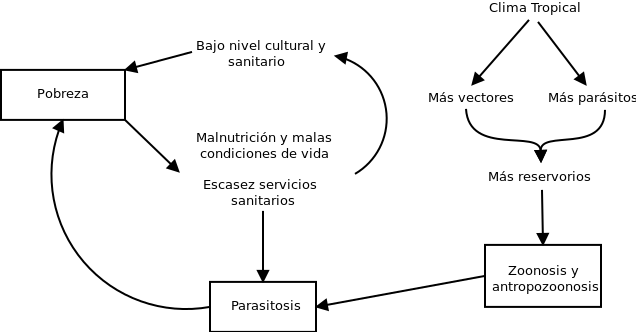
\includegraphics[width=\columnwidth]{figuras/ACV-BioSan-Parasit-ImportSocioecon}
		\caption{Esquema de las repercusiones socioeconómicas de las parasitosis.\label{fig:PARASIT:ConsecSocioecon}}
	\end{figure}
\end{multicols}
Las antropozoonosis suelen provocar rechazo social por confusión con otras patologías (\textit{Oncocerca volvulas} provoca dermatitis asemejan a la lepra), son incapacitantes, se asocian con profesiones o prácticas con rechazo social o manifestaciones que se asocian a prácticas calificadas como negativos o pensamientos magico-religiosos negativos o problemas de nutrición. Acaban, en infantes, generando retraso físico y mental. La mayor libertad sexual aumentó las parasitosis por vía venerea y ciertas inmunodepresiones (SIDA,etc.) y el aumento de intercambio de población y mercancías han aumentado la propagación de las parasitosis. El rechazo social incrementa el no tratamiento y con ello, contagio y propagación. Por ello, en tanto freno a la inversión, pérdida de productividad y aumento del gasto, las parasitosis generan subdesarrollo y este, retroalimenta el ciclo: la salud es necesaria para acabar con la pobreza.
\begin{figure}[H]
	\centering
	
\includegraphics[width=\columnwidth]{figuras/ACV-BioSan-Parasit-ImportSocioecon2}
	\caption{Consecuencias socioeconómicas que favorecen las parasitosis y efectos de estas.\label{fig:PARASIT:ConsecSocioecon2}}
\end{figure}
\chapter{\textit{Phylum} Protozoa}
\section{Sarcodinia}
\subsection{\textit{Entamoeba histolítica}}
Ameba cosmopolita, aunque con gran incidencia en regiones tropicales y subtropicales (prevalencia de hasta el 40 \%). Provoca, entre otras patologías, la \textit{diarrea del viajero}. Afecta a 10 millones de personas en todo el mundo, causando unas 100000 muertes anuales, siendo el 80 \% de los infectados portadores sanos. No obstante, la facilidad de confusión con \textit{Entamoeba dispar}, otra ameba comensal y no patógena, hace que los datos no sean del todo exactos. Se diferencian mediante técnicas de laboratorio (moleculares y bioquímicas).
\begin{multicols}{2}
	\subsubsection{Morfología}
	\textit{E. histolytica} presenta dos formas: una patógena (trofozoito) y otra de resistencia (quiste).
	\begin{itemize}[itemsep=0pt,parsep=0pt,topsep=0pt,partopsep=0pt]
		\item \textbf{Trofozoito}: (figura \ref{fig:PARASIT:EHistolyticaMorf}, derecha) sin forma constante por la emisión de pseudópodos, se meuve sobre superficies de forma directa por la emisión de lobópodos. Presenta dos zonas: ectoplasma (externo, de aspecto hialino y sin orgánulos celulares) y endoplasma (interno, rugoso y con orgánulos celulares). Tiene un núcleo con un nucleolo central y heterocromatina dispuesta perifericamente. En el citoplasma no se hallan mitocondrias, retículo endoplásmico o aparato de Golgi, pero sí polirribosomas, microtúbulos, glucógeno $\alpha \mbox{ o } \beta$ y vacuolas alimentarias con eritrocitos en degradación.
	\end{itemize}
	\columnbreak
	\begin{figure}[H]
		\centering
		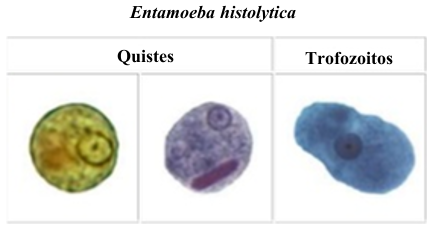
\includegraphics[width=0.9\columnwidth]{figuras/ACV-BioSan-Parasit-EHistolyticaMorf}
		\caption{\textit{E. histolytica} en sus dos morfologías: la de resistencia o quiste, con 2 ó 4 núcleos (inmaduros y maduros, respectivamente); y la forma patógena que se puede hallar en tejido.\label{fig:PARASIT:EHistolyticaMorf}}
	\end{figure}
\end{multicols}
\begin{itemize}[itemsep=0pt,parsep=0pt,topsep=0pt,partopsep=0pt]
	\item\textbf{Quistes}: (figura \ref{fig:PARASIT:EHistolyticaMorf}, central e izquierda) capaces de soportar las condiciones externas, es la forma de contagio. De forma esférica, presenta una membrana gruesa que lo protege y da forma. En su interior presenta 2 ó 4 núcleos, según su madurez (2, inmaduro; 4, maduro), acúmulos de glucógeno y unos cuerpos cromatoides en forma de huso (figura \ref{fig:PARASIT:EHistolyticaMorf}, central).
\end{itemize}
\begin{table}[H]
	\begin{tabular}{c|ccc}
		\rowcolor{black}&\textcolor{white}{\textit{\textbf{E. histolytica}}}&\textcolor{white}{\textbf{\textit{E. dispar}}}&\textcolor{white}{\textit{\textbf{E. coli}}}\\
		Tamaño quiste ($\mu m$)&15 a 20&15 a 20&15 a 50\\
		\rowcolor{hiperlightgray}Núcleos (en madurez)&4&4&8\\
		Nucleolo&Central&Central&Excéntrico\\
		\rowcolor{hiperlightgray}Cromatina&Uniforme&Uniforme&Irregular\\
		Cuerpos cromatoides& Bordes Redondeados&Bordes Redondeados&Bordes Astillados\\
		\rowcolor{hiperlightgray}Patogenicidad&Sí (hematófoga, con colonización extraintestinal)&No&No\\
		\hline
	\end{tabular}
	\caption{Diferencias morfológicas entre las principales \textit{Entamoebas} intestinales humanas.\label{table:PARASIT:EHistolyticaDiferMorf}}
\end{table}
\newpage
\begin{multicols}{2}
	\subsubsection{Ciclo biológico}
	Se trata de un ciclo directo, ocurriendo todo en un mismo hospedador. El punto de inicio del ciclo se da con la ingesta de agua y/o comida infectada con los quistes de \textit{E. histolytica}, ya sean maduros o inmaduros. Los quistes, por su tegumento, resisten los ácidos estomacales, produciendos la exquistación ante el pH neutro del intestino delgado. Se da una multiplicación nucleolar que resulta en un trofozoito multinucleado (con hasta 8 núcleos) que sufre una rápida citocinesis, obteniendo trofozoitos maduros que avanzan por el intestino empujados por el bolo alimenticio. A medida que descienden por el intestino, la menor humedad promueve el proceso de enquistación, formando un prequiste (se redondea y forma una cubierta glucídica que es la cubierta quística y se desorganiza el nucleolo), generando un prequiste con un núcleo y tras la cariocinesis, un quiste inmaduro, con la generación de los cuerpos cromatoides. La segunda cariocinesis da lugar a la maudración del quiste y pérdida de los cuerpos cromatoides. En las heces se expulsan todas las formas de estas amebas (los trofozoitos pueden desarrollar canales y proteínas que los unen a la pared intestinal y permiten invadirla), pero solo sobrevivirán los quistes. Existe también una via de infección por prácticas sexuales (oral o anal).
	\subsubsection{Puntos de control}
	\begin{itemize}[itemsep=0pt,parsep=0pt,topsep=0pt,partopsep=0pt]
		\item Saneamiento de aguas residuales
		\item Profilácticos.
		\item Medidas higienicas y lavado de alimentos (lejía alimentaria).
	\end{itemize}
	\columnbreak
	\begin{figure}[H]
		\centering
		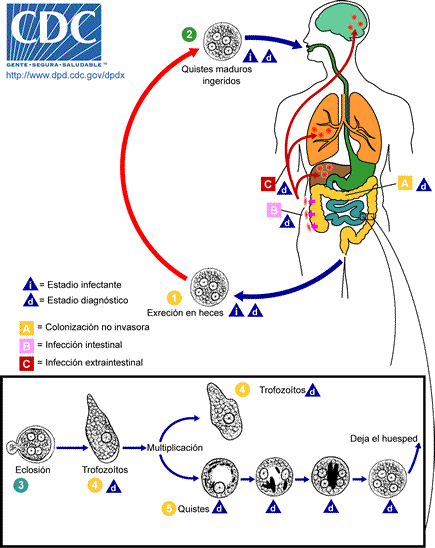
\includegraphics[width= \columnwidth]{figuras/ACV-BioSan-Parasit-EHistolyticaCbios}
		\caption{Ciclo biológico de \textit{E. histolytica}.\\Vehículo: agua o comida (directo no saprozoico).\\Vía: oral.\\Agente: quistes. \label{fig:PARASIT:EHistolyticaCBios}}
	\end{figure}
\end{multicols}
\subsubsection{Patología}
El periodo de incubación es de 2 a 21 días, el prepatente de 2 a 7 y el patente se puede extender durante años.
\begin{itemize}[itemsep=0pt,parsep=0pt,topsep=0pt,partopsep=0pt]
	\item\textbf{Disenteria\footnote{\textit{Muchas deposiciones}} amebiana} o \textbf{Amebiosis intestinal}: se produce en la fase inicial en el intestino. Los trofozoitos se adsorben en la mucosa y mediante enzimas, producen una actividad lítica del tejido, formando una úlcera <<en cuello de botella>>, reproduciendose en ella en forma de <<panal de abeja>>. Si la ulceración llega a la submucosa, pueden ir a localizaciones secundarias (enfermedad extraintestinal).
	\item\textbf{Amebomas}: granulomas en el cólon (sólo en el 1 \% de los casos, y en Latinoamérica).
	\item\textbf{Abcesos extraintestinales}: a través del torrente sanguineo, las amebas colonizan el SNC, hígado o lo hacen a través de las pleuras (con ulceraciones intestinales sangrantes).
\end{itemize}
\subsubsection{Sintomatología} 
\begin{itemize}[itemsep=0pt,parsep=0pt,topsep=0pt,partopsep=0pt]
	\item\textbf{Lesiones intestinales}: dolor abdominal; diarrea sanguinolienta , abunudante y con mucus; fiebre alta y dolor de cabeza. Si la amebiosis prospera, se pude producir paro cardiaco por agotamiento o peritonitis por perforación intestinal.
	\item\textbf{Lesiones extraintestinales}: se forman abcesos (formación con amebas externas e internas con tejido necrótico) en cerebro, bajo el nombre de meningoencefalitis amebiana secundaria; o abcesos hepáticos, en piel, pulmón y pene.
\end{itemize}
\subsubsection{Diagnosis}
\begin{itemize}[itemsep=0pt,parsep=0pt,topsep=0pt,partopsep=0pt]
	\item\textbf{Etiológico}: mediante examen de heces, distinguiendo a comensales como \textit{Entamoeba coli} o \textit{E. dispar}, esta última mediante técnicas moleculares.
	\item\textbf{Inmunodiagnóstico}: de escasa sensibilidad en caso de no haber amebas en sangre. Se hace mediante IFI, inmunohemoaglutinación, o ELISA (sensibilidad del 95 \% en casos extraintestinales, 70 \% en intestinales y 10 \% en asintomáticos; IgM dan positivo el 64 \% de las veces).
	\item\textbf{PCR}: permite descartar a \textit{E. dispar}.
\end{itemize}
\newpage
\section{Amebas anfiozoicas}
Las amebas anfizoicas\footnote{\textit{Ambas vidas} [libre y parasitaria].} siguen un ciclo biológico facultativo pudiendo vivir de forma exozoica como amebas de vida libre o endozoica como parasitos unicelulares. Su ciclo parasitario surge de una penetración accidental en el hospedador. Actualmente, se está dando un proceso de adaptación al parasitismo. Producen, por llevar acabo su acción primaria en el cerebro, una meningoencefalitis amebiana primaria que, por confusión en el diagnóstico y la falta de coevolución, resulta ser virulenta y mortal. Los géneros que afectan al ser humano son \textit{Naegleria fowleri}, \textit{Acanthamoeba cultbersoni}, \textit{Balamuthia} y \textit{Sappinia}; siendo las dos primeras las más incidentes.
\subsubsection{Morfología}
\begin{multicols}{2}
	\subsection{\textit{Naegleria fowleri}}
	Presenta tres estados. En todos los casos, el núcleo sólo es visible mediante microscopía de contraste de fases.
	\begin{itemize}[itemsep=0pt,parsep=0pt,topsep=0pt,partopsep=0pt]
		\item\textbf{Trofozoito ameboide}: muy activos metabolomicamente, no tienen forma constante por la emisión de pseudópodos, por los que se mueven por las superficies. Presentan un ectoplasma externo, hialino y sin orgánulos celulares; y un endoplasma interno, rugoso, con orgánulos celulares y el núcleo en posición central.
		\item\textbf{Trofozoito flagelado}: resultante del proceso a un medio líquido de las formas ameboides, o por medios poco ricos. Temporal, no presenta ectoplasma. Es ovalado, con endoplasma típico y dos flagelos polares.
		\item\textbf{Quistes}: capaces de soportar condiciones extremas, son redondeados, esféricos, con una membrana externa gruesa con perforaciones, núcleo central y endoplasma denso.
	\end{itemize}
	\columnbreak
	\subsection{\textit{Acanthamoeba cultbersoni}}
	Presenta dos estados:
	\begin{itemize}[itemsep=0pt,parsep=0pt,topsep=0pt,partopsep=0pt]
		\item\textbf{Trofozoito}: poco activo metabolicamente, sin forma constante, presenta un único núcleo y dos zonas diferenciadas: un ectoplasma externo, hialino y sin orgánulos celulares; y un endoplasma interno, rugoso, con orgánulos celulares. Tiene dos tipos de prolongaciones: filópodos, o pseudópodos espinosos, y acantopodinas, o lobópodos redondeados.
		\item\textbf{Quistes}: presenta las mismas estructuras del trofozoito (ectoplasma, endoplasma y un núcleo poco visible), carece de prolongaciones. El endoplasma tiene conformaciones poliédricas.
	\end{itemize}
\end{multicols}
\begin{figure}[H]
	\centering
	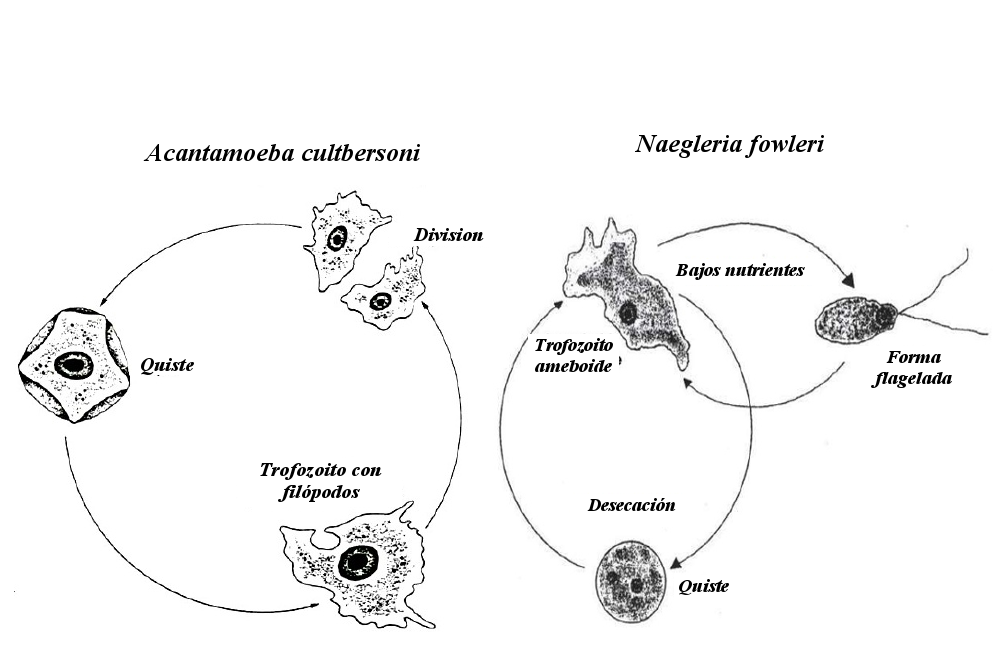
\includegraphics[trim=0 0.1cm 0.01cm 4cm,clip,width=0.65\columnwidth]{figuras/ACV-BioSan-Parasit-AAnfizMorf}
	\caption{Morfología y ciclo vital libre de las dos amebas anfizoicas más comunes: \textit{N. fowleri} y \textit{A. cultbersoni}.\label{fig:PARASIT:AAnfizMorf}}
\end{figure}
\subsubsection{Ciclo biológico}
Estas amebas se hallan presentes en el fondo de lagos y pozas (\textit{Naegleria} es capaz de vivir en aguas a 50º C y \textit{Acanthamoeba} vive en filtros de aire con \textit{L. pneumophila}). Estas amebas, por medio de turbulencias, ascienden a la superficie. Por aerosoles, estas amebas ingresan en la cavidad nasal del hospedador, llegando a su epitelio olfativo. De éste, siguiendo sus vías axonales, viajan al lóbulo olfativo, extendiendose por el encéfalo a la par que se multiplican asexualmente. En el caso de \textit{A. cultbersoni} puede llevar consigo a \textit{L. pneumophila}. Es capaz a su vez de introducirse por heridas en la piel o por la córnea.
\subsubsection{Puntos de control}
\begin{itemize}[itemsep=0pt,parsep=0pt,topsep=0pt,partopsep=0pt]
	\item Evitar bañarse en aguas no controladas.
	\item Cloración y salinización (>0.7 \%) de aguas.
	\item Adición de poliheximida al 2 \% para líquidos de lentillas.
\end{itemize}
\begin{figure}[H]
	\centering
	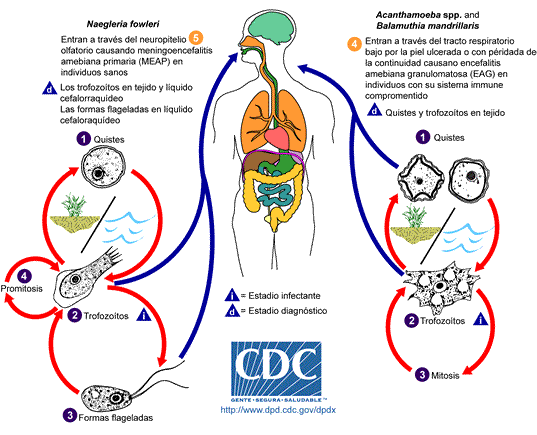
\includegraphics[width=0.72\columnwidth]{figuras/ACV-BioSan-Parasit-AAnfizCbios}
	\caption{Ciclos biológicos de \textit{N. fowleri} y \textit{A. cultbersoni}. Vehículo: aerosoles infectados (directo no saprozoicos), Vía: nasal, parenteral u ocular, Agente: Trofozoito.\label{fig:PARASIT:AAnfizCBios}}
\end{figure}
\subsubsection{Patología}
\begin{itemize}[itemsep=0pt,parsep=0pt,topsep=0pt,partopsep=0pt]
	\item\textbf{Meningoencefalitis amebiana primaria}: su periodo de incubación es de 1 a 3 días, o raramente de 7 a 14 días. La principal acción del parásito es una acción traumática de bloqueo, generando focos necróticos en el encéfalo. La sintomatología comienza con el comienzo de las divisiones y es facilmente confundible con una meningitis bacteriana: cefaleas, fiebre alta, nauseas, vómitos, rigidez de la nuca, encefalitis, creación de zonas necróticas y de consistencia blanda, meninges purulentas y congestión del bulbo olfativo. La muerte llega, en el 95 \% de los casos, a los 4 o 6 días.
	\item En el caso de \textit{A. cultbersoni}, causa:
	\begin{itemize}[itemsep=0pt,parsep=0pt,topsep=0pt,partopsep=0pt]
		\item\textbf{Encefalitis amebiana granulomatosa}: de desarrollo lento (periodo de incubación desconocido), se produce cuando el parásito se introduce por heridas y se distribuye por sangre. Allí donde se multiplica el parásito, forma una membrana. Los síntomas: afección nerviosa en varios puntos, dolor de cabeza insidioso, fiebre esporádica, ataxia y desorientación.
		\item\textbf{Queratinitis}: se produce ante situaciones de inmunocompromiso, traumas epiteliales en la córnea y agua de limpieza de lentillas contaminada con amebas. Se produce una destrucción de la córnea por inflamación, ulceración y perforación. Sus síntomas se confunden con infecciones por infecciones por herpes o bacterias: opacidad de la córnea, iritis, irritación ocular, lagrimeo excesivo, dolores agudos y pérdida de visión.
	\end{itemize}
\end{itemize}
\subsubsection{Diagnóstico}
\begin{multicols}{2}
	\subsubsection{\textit{Naegleria fowleri}}
	\begin{itemize}[itemsep=0pt,parsep=0pt,topsep=0pt,partopsep=0pt]
		\item\textbf{Clinico}: buscando síntomas y antecedentes del paciente.
		\item\textbf{Etiológico}: en líquido cefalorraquidio se puede encontrar viva y movil con Giemsa y tinciones de Wright. Cultivable en agar \textit{E. coli}.
		\item\textbf{Inmunológico}: Inmunofluorescencia o inmunoperoxidasa en necropsias.
		\item\textbf{PCR}.
	\end{itemize}
	\columnbreak
	\subsubsection{\textit{Acanthamoeba culbertsoni}}
	\begin{itemize}[itemsep=0pt,parsep=0pt,topsep=0pt,partopsep=0pt]
		\item\textbf{Etiológico}: se identifica en biopsias cutáneas o cerebrales (granulomas) o mediante su cultivo a 22 y 37º C.
		\item\textbf{Inmunológico}: mediante IFI o ELISA con antígenos extraidos de tejido fijados en formol.
		\item\textbf{PCR}.
	\end{itemize}
\end{multicols}
\newpage
\section{Ciliados}
\subsection{\textit{Balantidium coli}}
\section{Flagelados}
\subsection{\textit{Trypanosoma brucei}}
\subsection{\textit{Trypanosoma cruzi}}
\subsection{\textit{Leishmania} spp}
\subsection{\textit{Giardia lambia}}
\subsection{\textit{Trichomonas vaginalis}}
\section{Apicomplexa}
\subsection{\textit{Plasmodium} spp}
\subsection{\textit{Toxoplasma gondii}}
\subsection{\textit{Eimeria}}
\chapter{\textit{Phylum Plathelmintes}}
\section{Clase \textit{Cestoda}}
\subsection{\textit{Taenia saginata}}
\subsection{\textit{Taenia solium}}
\subsection{\textit{Hymenolepsis diminuta}}
\subsection{\textit{Hymenolepsis nona}}
\subsection{\textit{Diphilium caninum}}
\subsection{\textit{Echinococcus granulosus}}
\subsection{\textit{Diphylobotium latum}}
\section{Clase \textit{Trematoda}}
\subsection{\textit{Fasciola hepatica}}
\subsection{\textit{Fasciolopsis buski}}
\subsection{\textit{Clonorchis sinensis}}
\subsection{\textit{Schistosoma} spp}
\chapter{\textit{Phylum Nemathelmintes}}
\section{Superfamilia \textit{Filaroidea}}
\subsection{\textit{Wachereria bancrofti}}
\subsection{\textit{Dirofilaria inmitis}}
\section{Otras familias}
\subsection{\textit{Trichuris trichuria}}
\subsection{\textit{Trichinella spiralis}}
\subsection{\textit{Ancylostoma duodenale}}
\subsection{\textit{Ascaris lumbricoides}}
\subsection{\textit{Enterobius vermicularis}}
\chapter{\textit{Phylum Arthropoda}}
\section{Orden \textit{Anaplura}}
\subsection{\textit{Pediculus humanus}}
\subsection{\textit{Phtirius pubis}}
\section{Orden \textit{Siphonaptera}}
\subsection{\textit{Ctenofephlidus canis}}
\subsection{\textit{Pulex irritans}}
\section{Orden \textit{Diptera}}
\subsection{\textit{Anopheles} spp}
\subsection{\textit{Aedes} spp}
\subsection{\textit{Cules} spp}
\subsection{Suborden \textit{Cyclorrhopla}} %Stomxys, Musca, Colliplora, Callitroga, Sarcophaga, Gastrophilus, Hypoderma, Oestres
\section{Clase \textit{Arachnida}}
\subsection{\textit{Rhipicephtlus variablis}}
\subsection{\textit{Argus persicus}}
\part{Zoología}
\part{Metodologías de laboratorio}
\chapter{Técnicas electroquímicas}
\section{Medición de pH}
\chapter{Técnicas de separación de sustancias}
\section{Centrifugación}
\section{Electroforesis}
\subsection{Electroforesis en gel de agarosa}
\subsection{Electroforesis en gel de poliacrilamida}
\subsection{Electroforesis 2D}
\section{Cromatografía}
\subsection{Cromatografía plana}
\subsection{Cromatografía en columna}
\chapter{Espectrometría}
\section{Espectrofotometría visible y UV}
\section{Espectrometría de masas}
\section{Resonancia magnética nuclear}
\chapter{Métodos enzimáticos}
\section{Métodos enzimáticos colorimétricos}
\section{Zimografía}
\chapter{Técnicas inmunológicas}
\section{Inmunoprecipitación}
\section{Aglutinación y fijación del complemento}
\section{Inmunofluorescencia}
\section{Inmunoanálisis}
\subsection{Radioinmunoensayo (RIA)}
\subsection{ELISA}
\section{Inmunotransferencia: Western-blot}
\section{Inmunocitoquímica}
\subsection{Inmunocitoquímica directa}
\subsection{Inmunocitoquímica indirecta}
\section{Purificación de anticuerpos}
\subsection{Producción de anticuerpos monoclonales}
\section{Técnicas de determinación de complemento}
\chapter{Técnicas de Genética y Biología molecular}
\section{Aislamiento y purificación de ácidos nucleicos}
\subsection{Método de fenol-cloroformo-isoamílico}
\subsection{Método de isotiocianato de guanidina-fenol-cloroformo}
\section{Síntesis de ADNc: retrotranscripción}
\section{PCR}
\subsection{RT-PCR}
\subsection{PCR anidada}
\subsection{PCR múltiple}
\subsection{PCR \textit{in situ}}
\subsection{PCR cuantitativa en tiempo real}
\section{Clonación}
\section{Secuenciación}
\subsection{Método químico de Maxwell-Gilbert}
\subsection{Método enzimático de Sanger}
\subsection{Secuenciación automática}
\section{Southern-blot}
\section{Microarrays}
\section{RFLPs}
\section{MLPA}
\end{document}